\chapter{Analyse}
\label{ch:Analyse}
In diesem Kapitel werden zunächst einige verwandte Arbeiten vorgestellt und danach werden auf Basis dieser die Topologie, Protokolle und Messwerte für die Implementierungen dieser Arbeit ausgewählt.

\section{Verwandte Arbeiten} 
Die verwandten Arbeiten wurden in drei Unterkategorien unterteilt. 
Die erste Kategorie beschäftigt sich mit Selbstlokalisierung beziehungsweise indirekter Fernlokalisierung mittels IEEE 802.11.
Die Arbeiten der zweiten Kategorie basieren ebenfalls auf IEEE 802.11, hier wird jedoch eine Fernlokalisierung oder eine indirekte Selbstlokalisierung durchgeführt.
Die letzte Kategorie beschäftigt sich mit Arbeiten, die nicht auf IEEE 802.11 basieren, hier sind Verfahren beschrieben, die andere Protokolle verwenden.

\subsection{Verwandte Arbeiten - Selbstlokalisierung \& indirekte Fernlokalisierung mit IEEE 802.11}
Für die Selbstlokalisierung mit IEEE 802.11 werden auf der mobilen Einheit Messwerte für empfangene Pakete bestimmt und daraus die Position der mobilen Einheit berechnet.
Diese Information kann anschließend an einen Ortungsserver übertragen werden, dann handelt es sich um eine indirekte Fernlokaliserung.

\subsubsection{WiFi-LLS}
\label{ch:Vorherige:sec:LLS}
Chen et al. stellen mit dem WiFi-based Local Location System (WiFi-LLS) ein System zur indirekten Fernlokalisierung vor \cite{chen2007design}.
Als Messgröße wird die Stärke des empfangenen Signals (received signal strength, RSS) genutzt. 
Diese wird laut IEEE 802.11 Spezifikation als Index (RSSI) von der Hardware zurückgegeben. \\
Für die Ortung wird zunächst der RSSI von Paketen naher Access Points gemessen und zusammen mit der MAC-Adresse der mobilen Einheit in ein Paket gepackt und an den Ortungsserver versendet.
Anschließend wird auf dem Ortungsserver ein theoretisches Signalausbreitungsmodell $P(d) = P(d_0) - 10log_{10}(\frac{d}{d_0})^n - OAF$ mit der Distanz $d$, der Signalstärke $P(d)$ und der Referenzdistanz $d_0 = 1$m zur Bestimmung der Position der mobilen Einheit verwendet. \\
$P(d_0)$, der Pfadverlustexponent $n$ und der Hindernisdämpfungsfaktor $OAF$ müssen bestimmt werden, jedoch lassen sich $P(d_0)$ und $n$ auf einer einzelnen Teststrecke mit unterschiedlichen Abständen von AP und mobiler Einheit bestimmen. $OAF$ kann sogar für einen Gebäudetyp einmalig bestimmt werden.
Dadurch hat das Modell einen konstanten Aufwand. 
Dies ist für Baustellen interessant, da sich diese Werte einmalig messen und dann sogar über mehrere gleichartige Baustellen übertragen ließen.\\
In dieser Veröffentlichung steht die Ortungsgenauigkeit im Vordergrund und es werden keine Angaben zum Energieverbrauch gemacht. 
Als Referenz kann dienen, dass die mobile Einheit bei WiFi-LLS alle 5 Sekunden einen Scan (siehe Abschnitt \ref{ch:phase1:sec:scan}) durchführt, dann werden die Signalstärken entdeckter APs zusammen mit der eigenen MAC-Adresse in XML codiert und das so erzeugte Paket an den Ortungsserver versendet.

\subsubsection{AiRISTA Flow RTLS}
Ekahau bietet unter der Marke \textit{AiRISTA Flow RTLS} eine zu WiFi-LLS ähnliche Lösung kommerziell an \cite{airista2017airista}.
Ihr Ekahau B4 Badge Tag ermittelt regelmäßig den RSSI zu nahegelegenen APs und versendet diese an einen Ortungsserver \cite{liu2007survey}.
Das Tag bietet darüber hinaus noch einige Zusatzfunktionen, so können über die Datenverbindung auch Nachrichten und Alarmierungen an das Tag gesendet werden und die drei angebrachten Knöpfe können programmiert werden.\\
Bezüglich des Energieverbrauchs gibt sich das Informationsblatt des B4 Badge Tag vage: Das Tag soll abhängig vom Ortungsintervall wochenlang halten, danach muss der $600\ mA/h$ Akku geladen werden \cite{ekahau2017b4}.
Das Informationsblatt zum Ekahau W4, welches statt um den Hals am Handgelenk getragen wird, gibt an, dass der verbaute $530\ mA/h$ Akku bei einem Ortungsintervall von 15 Sekunden 500 Stunden (ca. 21 Tage) hält \cite{ekahau2017w4}.\\
AiRISTA Flow spricht auf ihrer Website zum Beispiel Krankenhäuser, Schulen und Regierungseinrichtungen an, hier sollen zusätzlich bewegliche Objekte, wie etwa Krankenhausbetten, geortet werden.
Die dazu verwendeten Asset Tags werden über einen Beschleunigungssensor aktiviert und können, wenn die Objekte selten bewegt werden, deutlich längere Laufzeiten erreichen \cite{ekahau2017a4}. \\
Im Umfeld des Tunnelbaus zeigte sich jedoch, dass die Tags keinesfalls wochenlange Laufzeiten aufwiesen, stattdessen entluden sie sich teilweise in unter zwölf Stunden.

\subsubsection{AeroScout}
Auch das AeroScout System von Stanley Healthcare richtet sich an den medizinischen Sektor und soll Objekte und Personen orten \cite{aeroscout2017asset}, \cite{aeroscout2017staff}.
Da sich auch dieses System in das bestehende WLAN-Netzwerk einfügt, sollte es ebenfalls auf einer indirekten Fernlokalisierung beruhen und demnach ähnliche Eigenschaften bezüglich des Energieverbrauchs aufweisen.\\
Das Informationsblatt ihres T14 Tags für Personen gibt eine Laufzeit von bis zu drei Wochen, abhängig von Konfiguration und Typ des Tags, an \cite{aeroscout2017t14}. 
Eine Angabe zu dem verwendeten Typ, der Konfiguration oder der Kapazität des verbauten Akkus wird nicht gemacht.\\

\subsubsection{Selbstlokalisierung mit Szenenanalyse}
\label{ch:Vorherige:sec:RSS-basierte}
Prasithsangaree et al. stellen ein System zur Selbstlokalisierung vor \cite{prasithsangaree2002indoor}, es verwendet aber eine offline-Phase zum Sammeln von Fingerabdrücken für Positionen in einem Abstand von 1,5 beziehungsweise 3 Metern. 
In diesen Fingerabdrücken werden die gemessenen RSSI der von den APs empfangenen Pakete als Merkmale zusammen mit der Position als Label gespeichert.
In der anschließenden online-Phase werden die gemessenen RSSI mit den Fingerabdrücken verglichen und die Position als gewichtetes Mittel der Labels bestimmt. \\
Die offline-Phase ist natürlich im Sinne der Aufgabenstellung nicht sinnvoll, da für eine Tunnelbreite von im Schnitt zehn Metern 4000 beziehungsweise 2000 Messungen pro Kilometer vorgenommen werden müssten.
Generell eignen sich Lösungen mit Szenenanalyse nicht gut für Baustellen, da diese nicht auf die potentiell höhere Genauigkeit angewiesen sind. 
Üblicherweise müssen dort sehr große Flächen vermessen werden und die Veränderungen durch den Baufortschritt führen dazu, dass regelmäßig neu gemessen werden muss.
Außerdem müssen bewegliche Störquellen wie Baumaschinen vorher aus dem Bereich entfernt werden, um unverfälschte Fingerabdrücke zu erhalten.
Der Aufwand ein System mit Szenenanalyse auf einer Baustelle zu betreiben ist deshalb sehr hoch und widerspricht der Forderung nach geringer Komplexität. \\
Die Arbeit zeigt aber die Volatilität der empfangenen Signalstärke auf, dies wurde 2011 von Lui et al. genauer untersucht \cite{lui2011differences}.
Lui et al. zeigen, dass die gemessene empfangene Signalstärke stark von der beteiligten Hardware abhängt und die Systeme jedes mal neu kalibriert werden müssen wenn sie auf ein neues AP-Modell portiert werden. 
Auf dem Areal sollte deshalb optimalerweise nur ein AP-Modell verwendet werden. \\
Abbildung \ref{fig:luiRSSI} zeigt die gemessenen RSSI Werte für die von ihnen getesten Netzwerkkarten mit unterschiedlichen Distanzen, für einige Karten korreliert die empfangene Signalstärke nur sehr schwach mit der Distanz zwischen Basisstation und mobiler Einheit.
Sie zeigen außerdem, dass einige AP-Modelle den RSSI speichern und nur bei größeren Veränderungen aktualisieren und dass die Antenne signifikanten Einfluss auf den protokollierten Wert hat.

\begin{figure}[h]
  \centering
	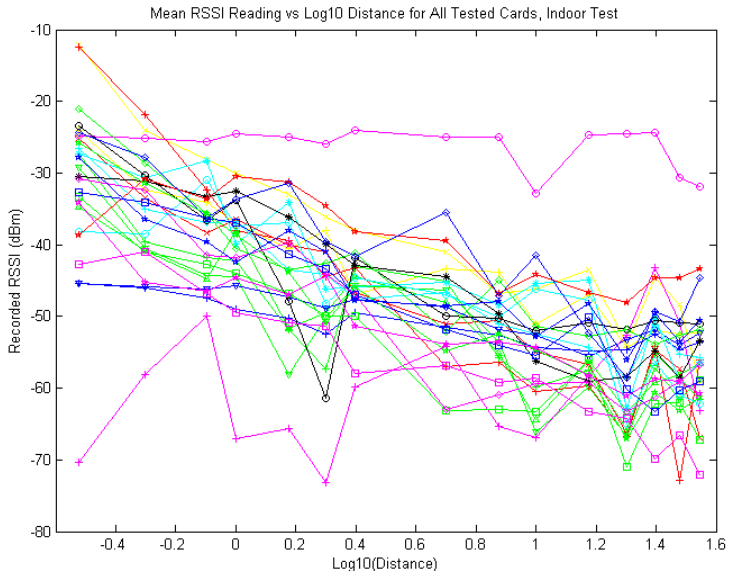
\includegraphics[width=\textwidth]{images/luiRSSI.png}
  \caption{Gemessener RSSI mit verschiedenen Access Points und Distanzen, aus \cite{lui2011differences}.}
  \label{fig:luiRSSI}
\end{figure}




\subsection{Verwandte Arbeiten - Fernlokalisierung \& indirekte Selbstlokalisierung mit IEEE 802.11}
Für die Fernlokalisierung mit IEEE 802.11 werden auf den Basisstationen Messwerte für empfangene Pakete bestimmt und daraus die Position der mobilen Einheit berechnet.
Diese Information kann anschließend an die mobile Einheit übertragen werden, dann handelt es sich um eine indirekte Selbstlokaliserung.

\subsubsection{RADAR}
\label{ch:Vorherige:sec:RADAR}
Das RADAR System von Bahl et al. (Microsoft Research) hat als eins der ersten WLAN-basierten Ortungssysteme viel Aufmerksamkeit erfahren \cite{bahl2000radar}.
Als Messgröße wird die Stärke des empfangenen Signals (received signal strength, RSS) genutzt, diese wird laut IEEE 802.11 Spezifikation als Index (RSSI) von der Hardware zurückgegeben. 
Das RADAR System ist auf eine offline-Phase angewiesen, in der empirisch ein Signalausbreitungsmodell aufgebaut wird. 
Es handelt sich also um ein System mit Szenenanalyse.\\
Die Verwendung einer offline-Phase ist im stark veränderlichen Baustellenumfeld nicht akzeptabel. 
Zum einen führt der ständige Baufortschritt dazu, dass regelmäßig neu kalibriert werden muss und zum anderen wirken sich auch die großen Baumaschinen auf die Signalausbreitung aus. 
Damit sich dies nicht im Modell wiederfindet, müssten zunächst alle beweglichen Maschinen aus dem Bereich entfernt werden, um anschließend in der online-Phase ihren Einfluss glätten zu können.
Die offline-Phase ist deshalb wirtschaftlich gesehen nicht durchführbar und das empirisch ermittelte Signalausbreitungsmodell müsste durch ein theoretisches ersetzt werden, für eine grobkörnige Bereichsortung sollte dies jedoch ausreichend sein.\\
Bei RADAR sendet die mobile Einheit vier UDP-Pakete pro Sekunde aus, an den Basisstationen wird dann der RSSI gemessen.
Die Autoren weisen jedoch darauf hin, dass sich dieser Vorgang leicht umkehren ließe, um von einer Fernlokalisierung auf eine Selbstlokalisierung zu kommen.
Bezüglich des Energieverbrauchs äußern sie sich jedoch zu keiner der beiden Varianten.\\
Die Position wird anschließend bestimmt, indem aus den in der offline-Phase aufgenommenen Werten derjenige mit dem geringsten Abstand zu den gemessen Werten gewählt wird. 
Dies wird im \textit{nearest neighbour in signal space (NNSS)} Algorithmus beschrieben.
Für die Ortung wird mehrfach gemessen und dann gemittelt, um im Median eine Genauigkeit von unter 3 Metern zu erhalten. 
Das kurze Sendeintervall von 0,25 Sekunden führt auch bei bewegten Personen zu einer Genauigkeit von 3,5 Metern.
Gleichzeitig sorgt das kurze Sendeintervall aber auch für einem hohen Energieverbrauch auf Seiten der mobilen Einheit, eine Reduktion der Sendevorgänge sollte im Kontext der Bereichsortung angestrebt werden, um den Energieverbrauch zu senken und die Batterielaufzeit der mobilen Einheit zu steigern.

\subsubsection{Verbesserungen an RADAR}
Bahl et al. veröffentlichten anschließend noch einige Verbesserungen für das ursprüngliche RADAR System \cite{bahl2000enhancements}.
Diese umfassen unter anderem den Einsatz von Access Points statt PCs als Basisstationen, verbesserte Ortung bewegter Personen und die Erkennung von hinzugekommenen Hindernissen wie etwa Personen.
Letzteres geschieht durch die Analyse der Signalstärke von Beacons anderer APs, da diese sich nicht bewegen, können Veränderungen in der Signalstärke als Veränderungen auf dem Signalweg gesehen werden.
Dies ließe sich auch auf größere Hindernisse übertragen, hängt aber stark von der strategischen Platzierung und möglichst dichten Verteilung der APs ab.\\
Auch hier äußern sich die Autoren nicht zum Energieverbrauch, wohl auch deshalb weil sie einen Laptop als mobile Einheit verwenden.

\subsubsection{Time-of-flight Lokalisierung}
\label{ch:Vorherige:sec:TOF}
Aufgrund der Schwächen von RSS-basierten Systemen wurde auch über solche nachgedacht, die stattdessen oder zusätzlich die time-of-flight (TOF) messen. 
Ein Beispiel für ein solches zeigen Wibowo et al. \cite{wibowo2009time}. 
Sie fordern optimalerweise Zugriff auf die physische Schicht (PHY) des IEEE 802.11 Protokolls, da auf diesen aber üblicherweise kein Zugriff besteht, messen sie TOF in der darüber liegenden MAC-Schicht.\\
Eine Basisstation sendet einen Beacon aus und protokolliert die Sendezeit, die mobile Einheit empfängt den Beacon, protokolliert die Empfangszeit und die Sendezeit der gesendeten Antwort, die Basisstation sichert die Empfangszeit der Antwort.
Nun sendet die mobile Einheit die zwei gespeicherten Zeitstempel an die Basisstation, der mit diesen die Verarbeitungszeit auf der mobilen Einheit berechnen kann, um dann die Distanz $d = c * (\frac{t_{empfangen} - t_{gesendet} - t_{Verarbeitung}}{2})$ zur mobilen Einheit zu bestimmen.
Dieses Schema lässt sich leicht von einer Fernlokalisierung in eine Selbstlokalisierung umwandeln, indem man den Initiator des Vorgangs tauscht.\\
Die Notwendigkeit die Zeitstempel bereits in der PHY- beziehungsweise MAC-Schicht zu setzen erfordert Zugriff auf die Software des als Basisstation verwendeten Access Points. 
Außerdem müssen die Zeitstempel im Bereich von Nanosekunden gesetzt werden und die Verarbeitungszeit vor/nach dem Setzen muss sehr konstant sein, da eine Abweichung von 100 ns bei c = 299.792.458 m/s bereits einen Fehler von 30 Metern verursacht.\\
Muthukrishnan et al. beschreiben diese Problematik bei dem Versuch TOF ohne Zugriff auf die Software des APs umzusetzen \cite{muthukrishnan2006using}.
Sie kommen zu dem Ergebnis, dass sich die in der Spezifikation eingebauten Zeitstempelfunktionen wie das Network Time Protocol (NTP), Ping und die Zeitstempel in Beacons nicht eignen, da sie zum einen nur eine Auflösung im Millisekundenbereich bieten und zum anderen von der Blockierungskontrolle von IEEE 802.11 (CSMA/CA) abhängen.

\subsubsection{Ortung ohne mobile Einheit}
Eine Ortung ohne mobile Einheit erfüllt wegen ihrer Abwesenheit offensichtlich jede Anforderung an die Batterielaufzeit der mobilen Einheit.
Mit MonoPHY stellen Abdel-Nasser et al. ein System zur Ortung ohne mobile Einheit vor \cite{abdel2013monophy}. \\
Dazu verwenden sie einen IEEE 802.11n-fähigen Laptop und Access Point und analysieren die Channel State Information (CSI) der physischen Schicht (PHY) der zwischen AP und Laptop übertragenen Daten.
Um die bestehende Struktur von APs zu nutzen, sollte das System angepasst und die CSI zwischen den APs gemessen werden.
Es hat jedoch einige Aspekte, die es ungeeignet für die Aufgabenstellung machen.\\
Das System unterscheidet nicht zwischen Personen, sondern erkennt nur, dass jemand anwesend ist. 
Außerdem ist es nur für eine Person in einem 100 $m^2$ Apartment gestaltet worden und müsste auf Baustellengröße und die Verfolgung vieler Personen erweitert werden.
Aber auch dann ist fraglich, wie gesichert werden kann, dass alle Personen durchgehend erkannt werden können, zum Beispiel wenn sich mehrere Personen auf oder in einem Transportfahrzeug aufhalten.
Auch ist es ohne Identifikation schwerer Fehler zu erkennen. 
Wird fälschlicherweise angezeigt, dass sich noch eine Peron im Tunnel befindet, kann oft durch ausrufen des Betreffenden festgestellt werden, dass dieser nicht im Tunnel ist. 
Hat man dagegen nur die Information, dass sich noch eine Person im Tunnel befindet, hat man keine Möglichkeit schnell herauszufinden ob dies der Wahrheit entspricht.\\
Weitere Probleme entstehen durch die Baumaschinen und Container. 
Diese haben einen starken Einfluss auf die CSI und verdecken dadurch möglicherweise nahe Personen und die Fahrzeugführer.
Deshalb müssten diese Objekte ebenfalls als Entitäten angezeigt werden. 
Die Anzeige diverser Kommandostände, Pausenräume und stehen gelassener Baumaschinen verwirrt im Notfall jedoch, da sich in jedem Objekt potentiell eine Person befinden könnte.\\
Die Veröffentlichung beruht außerdem auf der Verfügbarkeit der CSI, diese sind dort durch die Auswahl einer bestimmten Netzwerkkarte gegeben und sind nicht zwingend in einer bestehenden Struktur von APs verfügbar.
Als letzter Kritikpunkt steht die Verwendung eine offline-Phase, die, wie bereits diskutiert, wirtschaftlich nicht umsetzbar ist. \\ 
Somit erfüllt die Ortung ohne mobile Einheit zwar die Anforderungen an den Energieverbrauch, jedoch nicht die Forderung nach sicherer Erkennung von Abschnittswechseln, deshalb scheidet diese Technik zumindestens für Baustellen aus.




\subsection{Verwandte Arbeiten - Funkbasierte Lokalisierung mit weiteren Funkprotokollen}
Die Arbeiten in dieser Kategorie verwenden nicht IEEE 802.11 für die Lokalisierung.
Sie verwenden stattdessen andere Protokolle, die sich durch einen geringeren Energieverbrauch als IEEE 802.11 auszeichnen sollen.

\subsubsection{Geeignete Messwerte für Bluetooth}
Hossain et al. untersuchen die laut Bluetooth Spezifikation zurückgegebenen Messwerte bezüglich ihrer Eignung für die Lokalisierung \cite{hossain2007comprehensive}.\\ 
Link Quality (LQ) beschreibt, wie gut die Verbindung zwischen zwei Geräten ist.
Der Wert wird aus der Bitfehlerrate beim Empfänger berechnet, allerdings ist nicht spezifiziert, wie der Wert zu berechnen ist, er hängt also in hohem Maße vom Hersteller des Empfängers ab. \\
Der Received Signal Strength Indicator (RSSI) misst die Stärke des eingehenden Signals, die Spezifikation sieht jedoch eine Golden Receive Power Range (GRPR) vor. 
Liegt der RSSI über oder unter dieser wird eine Anfrage zum erhöhen oder verringern der Sendeleistung an das andere Gerät verschickt, dies dient während einer aktiven Verbindung dazu den Energieverbrauch zu senken.
Problematisch am RSSI ist, dass er relativ zur GRPR bestimmt wird.
In der Untersuchung von Hossain et al. führte das dazu, dass der RSSI mit 0 gemessen wurde, wenn er innerhalb der GRPR lag. \\
Transmission Power Level (TPL) ist die Sendeleistung eines Geräts. 
TPL kann während einer bestehenden Verbindung durch Anfragen des Verbindungspartners verändert werden.
Dazu muss diese Energiesparfunktion jedoch unterstützt werden, was bei dem von Hossain et al. verwendeten Gerät nicht der Fall war.
Abbildung \ref{fig:bluetoothmess} zeigt deshalb für TPL eine waagerechte Linie.\\
Für Inquirys wird die Stärke des eingehenden Signals ohne die Beachtung des GRPR bestimmt.
Außerdem werden Inquirys immer mit voller Sendeleistung gesendet, da sie zur Entdeckung von Ressourcen verwendet werden.
Es handelt sich ebenfalls um den RSSI, um jedoch den Unterschied zum RSSI für eine Verbindung deutlich zu machen nennen Hossain et al. diesen Wert RX Power Level.

\begin{figure}[h]
  \centering
	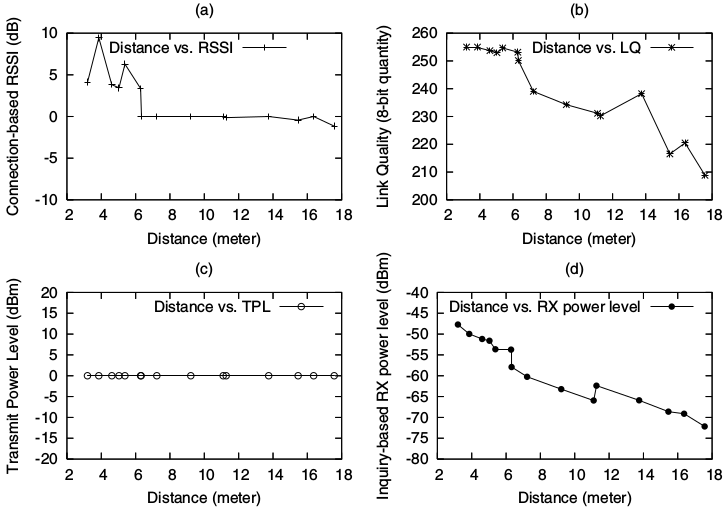
\includegraphics[width=\textwidth]{images/bluetoothmess.png}
  \caption{Korrelation der Messwerte mit der Distanz, aus \cite{hossain2007comprehensive}}
  \label{fig:bluetoothmess}
\end{figure}

\subsubsection{Antwortbasierte Inquiry Lokalisierung}
Bargh et al. stellen ein System zur Fernlokalisierung mittels Bluetooth Inquiry Scan vor \cite{bargh2008indoor}.
Die mobilen Einheiten sind dabei im discoverable ("{}entdeckbar"{}) Modus.
Die Basisstationen senden regelmäßig eine Inquiry Message aus, die dann von mobilen Einheiten in Reichweite mit einer Inquiry Response beantwortet werden. 
Anschließend werden die Antworten auf einem zentralen Ortungsserver gesammelt und die Positionen der mobilen Einheiten bestimmt.
Diese Information wird aus den beantworteten Inquiry Messages jeder mobilen Einheit gewonnen.
Dazu werden vorher in einer offline-Phase Fingerabdrücke für jeden Raum gesammelt.
In diesen wird gespeichert welche Inquiry Messages von der mobilen Einheit an einem bestimmten Ort beantwortet wurden.
Für die Bereichsortung entfiele diese offline-Phase, da der Bereich über die Beantwortung einer einzelnen Inquiry Message implizit bestimmt werden kann.
Tabelle \ref{table:irr} zeigt die abnehmende Warscheinlichkeit für eine Antwort auf die Inquiry Message mit steigender Distanz.

\begin{table}[h]
  \centering
  \caption{Rate der beantworteten Inquiry Messages (Inquiry Response Rate, IRR) gegen Distanz, aus \cite{bargh2008indoor}}
	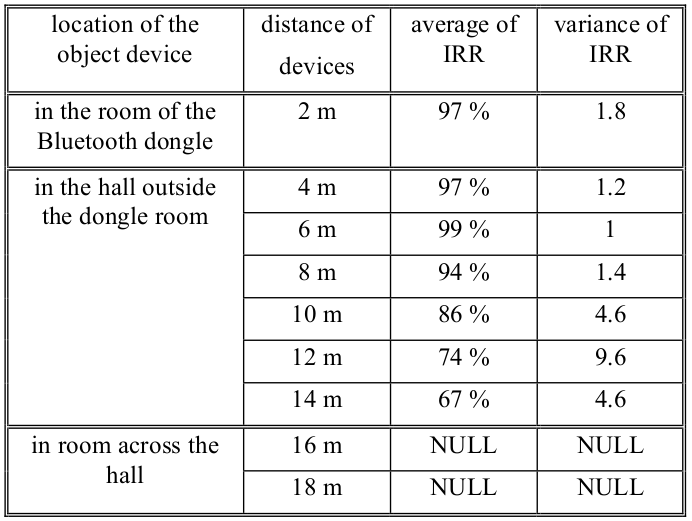
\includegraphics[width=0.7\textwidth]{images/irr.png}

  \label{table:irr}
\end{table}

\subsubsection{RSSI-basierte Inquiry Lokalisierung}
Ling et al. lokalisieren Bluetooth-fähige Geräte über den RSSI der Inquiry Response \cite{ling2010inquiry}.
Ihre Basisstationen versenden regelmäßig Inquiry Messages und messen den RSSI der Inquiry Responses.
Mobile Einheiten, die geortet werden wollen beziehungsweise sollen, bewerben in der Inquiry Response einen speziellen Service.
Dies erlaubt es diese herauszufiltern und die Privatsphäre anderer Personen zu wahren.
Die Autoren verwenden eine anfängliche offline-Phase um Fingerabdrücke für den RSSI an gegebenen zu finden.
Allerdings messen sie dazu an den Basisstationen die empfangene Signalstärke von Übertragungen anderer Basisstationen, folglich kann die offline-Phase automatisiert durchgeführt werden.
Für die online-Phase werden die gemessenen RSSI Werten über eine Warscheinlichkeitsverteilung geglättet, um eine bessere Ortungsgenauigkeit zu erreichen.
Für die eigentliche Lokalsierung werden die gemessenen RSSI mit den Warscheinlichkeitsverteilungen aus der offline-Phase verglichen und die Warscheinlichkeit für die Emission dieser Werte über die Position maximiert.

\subsubsection{RSSI-basierte BLE Lokalisierung}
Jianyong et al. stellen ein System zur Lokalisierung auf Basis von Bluetooth Low Energie (BLE, auch Bluetooth Smart) vor \cite{jianyong2014rssi}. \\
Sie messen an den Basisstationen den RSSI von Advertising Paketen, die zuvor von den mobilen Einheiten versendet wurden.
Für die genaue Ortung werden die Ergebnisse mit einem Gauß-Filter geglättet und für jede Basisstation die Parameter für ein Signalausbreitungsmodell bestimmt.
Die gemessene Signalstärke $P = A - 10n*log(d)$ hängt von der Referenzsignalstärke A im Abstand von einem Meter, dem Dämpfungsfaktor n und der Distanz d ab. \\
Jianyong et al. bestimmen die Referenzsignalstärke und den Dämpfungsfaktor für jede Basisstation.
Da jedoch nur eine Bereichsortung für diese Arbeit gefordert wurde, sollten A und n nur beispielhaft für eine Basisstation bestimmt werden, um den Aufwand beim Aufbau der Infrastruktur zu reduzieren.
Abbildung \ref{fig:blemodel} zeigt die von Jianyong et al. bestimmten Parameter für das Signalausbreitungsmodell. 
Abbildung \ref{fig:blemodel} zeigt außerdem, dass die verwendeten CC2540 Development Kit von Texas Instruments von einer Basisstation nur auf 20 Meter detektiert werden konnte.


\begin{figure}[h]
  \centering
	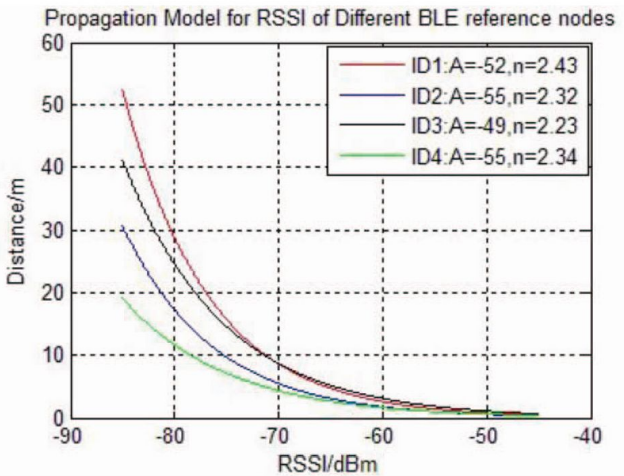
\includegraphics[width=0.7\textwidth]{images/blemodel.png}
  \caption{Signalausbreitungsmodelle aus \cite{jianyong2014rssi}}
  \label{fig:blemodel}
\end{figure}

\subsubsection{Lokalisierung mit LoRa}
Kim et al. stellen ein System zur Lokalisierung mit LoRa vor \cite{kim2016poster}.
Sie beziehen sich dabei auf eine Lokalisierung im Außenbereich in einem 30x30km Areal. 
Sie senden Pakete von der mobilen Einheit und messen die Time of Arrival (ToA) an den Basisstationen.
Dazu müssen die Basisstationen zeitsynchron arbeiten, dies wird über GPS sichergestellt.\\
Eine Lokalisierung über den RSSI lehnen sie ab, da dieser im Bereich von 20 bis 30km Entfernung nur um 3-6dBm fällt und die Varianz die Korrelation von RSSI und Distanz über lange Distanzen überdeckt.
Sie erreichen, abhängig von der Anzahl der verwendeten Basisstationen eien Genauigkeit zwischen wenigen Hundert und fast eintausend Metern, siehe dazu Abbildung \ref{fig:loraacc}

\begin{figure}[h]
  \centering
	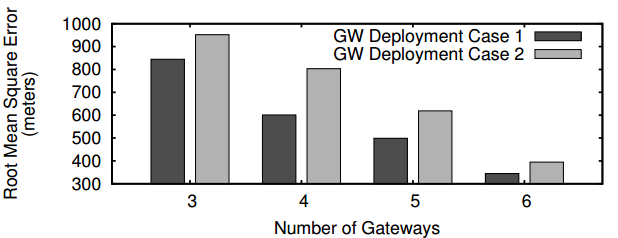
\includegraphics[width=0.7\textwidth]{images/loraacc.png}
  \caption{Quadratischer Fehler der Lokalisierung aus \cite{kim2016poster}, Gateways stellen Basisstationen dar.}
  \label{fig:loraacc}
\end{figure}

\section{Auswahl des Funkprotokolls}
Soll das bestehende WLAN Netzwerk genutzt werden ist die Wahl auf die IEEE 802.11 Spezifikation beschränkt.\\
Kann man aber die Hardware für die Basisstationen frei wählen, kann auch das Protokoll frei gewählt werden.
Es werden deshalb zusätzlich BLE und LoRa betrachtet.\\
Bluetooth Low Energy wird gegenüber normalem Bluetooth aufgrund seiner Charakteristik als Protokoll für geringen Energieverbrauch bevorzugt.\\
LoRa bietet zwar theoretisch eine sehr hohe Reichweite, diese ist jedoch stark von verwendeten Antennen und den Hindernissen abhängig.
Ob LoRa einen signifikanten Vorteil bei der Reichweite hat muss geprüft werden.
Sollte dieser Vorteil bestehen, bietet LoRa durch seine bessere Abdeckung eine höhere Sicherheit bei der Erkennung von Abschnittswechseln. 
Außerdem ist es dadurch potentiell möglich auf triangulierte Positionen zu wechseln ohne mehr Basisstationen aufbauen zu müssen.

\section{Auswahl der Topologie}
Das Wissen um die Position der Nutzer soll nach der Ortung dem Sicherheitssystem der Baustelle zur Verfügung stehen. 
Das Sicherheitssystem fungiert daher konzeptionell auch als zentraler Ortungsserver.
Es muss deshalb eine Fernlokalisierung durchgeführt werden, diese kann aber sowohl direkt als auch indirekt durchgeführt werden. \\
Weil laut IEEE 802.11 keine für die Lokalisierung geeigneten Messwerte vom AP in das angeschlossene Netzwerk propagiert werden, kommt keine der verwandten Arbeiten zur direkten Fernlokalisierung mit IEEE 802.11 ohne Zugriff auf die Software des AP aus.
Es werden deshalb sowohl die direkte, als auch die indirekte Fernlokalisierung mit IEEE 802.11 untersucht, obwohl eine Lösung mit indirekter Fernlokalisierung wegen des nötigen Empfangs von Signalen potentiell mehr Energie verbraucht.\\
Dürfen Veränderungen der Hardware vorgenommen werden, bietet sich ebenfalls eine direkte Fernlokalisierung an, da dort die mobilen Einheiten, abgesehen von der Kollisionsdetektion/-vermeidung, nicht empfangen müssen.\\
Eine Topologie ohne Basisstationen kommt nicht in Frage, da diese Topologie Einzelpersonen insbesondere in Notsituationen nicht ausreichend gut erfasst.




\section{Auswahl der Messgrößen}
Da nur eine Bereichsortung durchgeführt werden soll, sind die Anforderungen an die erzielte Genauigkeit gering.
Stattdessen sollte darauf geachtet werden, dass die Anforderung für die Messung gering ist.
Messgrößen, die Zeitsynchronität vorraussetzen sind daher nicht geeignet.\\
Als Messgröße wird der Received Signal Strength Index für alle drei Technologien gewählt, da dieser bei jedem empfangenen Paket von der physischen Schicht gemessen und am empfangenden Gerät leicht ausgelesen werden kann.\\
Auch bei LoRa wird der RSSI entgegen der Empfehlung von Kim et al. gewählt.
Da sich das Szenario im Gegensatz zu dem aus ihrer  Veröffentlichung unter Tage abspielt kann keine Synchronisierung über GPS gewährleistet werden. 
Außerdem müssen die Distanzen zwischen den Basisstationen geringer gewählt werden, da die Ungenauigkeiten aus dieser Veröffentlichung zu hoch für das Szenario sind.

\section{Auswahl der Hardware}
Die verwendeten Radios müssen die physische Schicht des jeweils verwendeten Protokolls beherrschen.
Es werden deshalb Radios für 802.11, Bluetooth 4.0 oder höher und LoRaWan benötigt.\\
Die Feather-Serie von Adafruit beinhaltet viele eigenständige Entwicklungs-Boards, darunter finden sich für jede der benötigten Funktechnologien ein Entwicklungs-Board.
Das \textit{Adafruit Feather HUZZAH ESP8266} wird für mobile Einheiten mit IEEE 802.11 eingesetzt.
Mobile Einheiten mit Bluetooth werden mit dem \textit{Adafruit Feather nRF52 Bluefruit} implementiert, es unterstützt Bluetooth 5.0 inklusive BLE.
Unterstützung für LoRa bietet das \textit{Adafruit Feather M0 RFM95 LoRa Radio (900MHz)}, mit diesem werden mobile Einheiten mit LoRa implementiert.\\

\section{Weiteres Vorgehen}
Im Folgenden werden Prototypen für die drei ausgewählten Protokolle erstellt, IEEE 802.11 ist dabei in indirekte und direkte Fernlokalisierung geteilt, da die direkte Fernlokalisierung Zugriff auf die Software der Basisstationen erfordert.
Zusätzlich wird die Reichweite jeder Funktechnologie im Tunnel überprüft, da diese für das Intervall der Ortungsvorgänge und die Ekennungssicherheit wichtig ist.
Abschließend werden in jedem Kapitel die Charakteristika des Stromverbrauchs der jeweiligen mobilen Einheiten überprüft.
